\documentclass[a4paper,14pt]{article}

\input{lab_Preamble.tex}


\begin{document}
\author{Рябых Владислав и Исыпов Илья, Б05-905}
\title{\tbf{3.4.1.(4.13) Измерение магнитной восприимчивости диа- и парамагнетиков}}
\maketitle

Цель работы: измерение магнитной восприимчивости диа- и парамагнитного образцов.

В работе используются: электромагнит, аналитические весы, милливеберметр, источник питания постоянного тока, образцы диа- и парамагнетиков.


\section*{Теория}
Магнитная восприимчивость тел может быть определена методом измерения сил, действующих на тела в магнитном поле. В данной лабораторной работе магнитная восприимчивость образцов будет измерена по методу Гюи: используется тонкий и длинный стержень, один из концов которого помещается в зазор электромагнита (обычно в область однородного магнитного поля), а другой конец помещается в область пространства, где влиянием магнитного поля можно пренебречь. Закон изменения поля -- от максимального до минимального значения в данном случае не существенен. 

\begin{figure}[bhtp]
	\centering
	\includegraphics[width=0.3\linewidth]{first}
	\caption{расположение образца в зазоре электромагнита}
\end{figure}
	
	Найдем выражение для магнитной силы, действующей на такой образец (рис. 1). Пусть площадь образца равна $s$, его магнитная проницаемость -- $\mu$, а поле в зазоре равно $B$.
	Воспользуемся для расчёта энергетическими соображениями. Магнитная сила может быть вычислена как производная от магнитной энергии по перемещению. Из теории известно, что эту производную следует брать со знаком минус, когда образец находится в поле постоянного магнита, или со знаком плюс, как в нашем случае, когда образец находится в поле в зазоре электромагнита, ток $I$ в обмотках которого поддерживается постоянным.

При смещении образца на $\Delta l$ вниз магнитная сила, действующая на него равна:

\begin{equation}
	F = \left( \dfrac{\Delta W_{\text{м}}}{\Delta l}\right)_I,
\end{equation}
где $\Delta W_{m}$ -- изменение магнитной энергии системы при постоянном токе в обмотке электромагнита и, следовательно, при постоянной величине магнитного поля в зазоре.

Магнитная энергия рассчитывается по формуле:

\begin{equation}
	W_{m} =  \dfrac{1}{2} \int H B dV = \dfrac{1}{2\mu_0}  \int \dfrac{B^2}{\mu} dV,
\end{equation}
где интеграл распространен на все пространство. При смещении образца, магнитная энергия меняется только в области зазора (в объеме площади $s$ и длины $\Delta l$), около верхнего конца стержня остается неизменной, поскольку магнитного поля там практически нет. Принимая поле внутри стержня равным измеренному нами полю в зазоре $B$ получим

\begin{equation*}
    \Delta W_{m} = \dfrac{1}{2\mu_0}\cdot\dfrac{B^2}{\mu}s\Delta l - \dfrac{1}{2\mu_0}\cdot B^2 s\Delta l = \dfrac{1 - \mu}{2\mu_0 \mu}\cdot B^2 s\Delta l = -\dfrac{\chi}{2\mu_0 \mu}\cdot B^2 s\Delta l.
\end{equation*} 
Следовательно, на образец действует сила:

\begin{equation}
	F = -\dfrac{\chi}{2\mu_0 \mu}\cdot B^2 s, 
\end{equation}

Знак силы, действующей на образец зависит от знака $\chi$: образцы из парамагнитных материалов ($\chi > 0$) втягиваются в зазор электромагнита, а диамагнетики ($\chi < 0$) выталкиваются из него.

Пренебрегая отличием $\mu$ от единицы, получаем окончательную расчётную формулу в виде

\begin{equation}
F = -\dfrac{\chi B^2 s}{2\mu_0}, 
\end{equation}\

Измерив силу, действующую на образец в магнитном поле $B$ можно рассчитать магнитную восприимчивость образца.

\section*{Экспериментальная установка}
\begin{figure}[!h]
 	\centering
	\includegraphics[width = 8cm]{second}
	\caption{Схема экспериментальной установки}
\end{figure}

Схема установки приведена на рис. 2. Магнитное поле с максимальной индукцией $\simeq 1$ Т создается в зазоре электромагнита, питаемого постоянным током. Диаметр полюсов существенно превосходит ширину зазора, поэтому поле в центре зазора достаточно однородно. Величина тока, проходящего через обмотки электромагнита, регулируется при помощи источника питания GPR и измеряется амперметром А, встроенным в источник питания. Градуировка электромагнита (связь между индукцией магнитного поля $B$ в зазоре электромагнита и силой тока $I$ в его обмотках) производится при помощи милливеберметра. 

При измерениях образцы поочередно подвешиваются к аналитическим весам так, что один конец образца оказывался в зазоре, а второй -- вне зазора, где индукцией магнитного поля можно пренебречь. При помощи аналитических весов определяется перегрузка $\Delta P = F$ -- сила, действующая на образец со стороны магнитного поля.

Силы, действующие на диа- и парамагнитные образцы, очень малы. Небольшие примеси ферромагнетиков (сотые доли процента железа или никеля) способны кардинально изменить результат опыта, поэтому образцы были специально отобраны.

\section*{Ход работы}
Проведем калибровку магнита. Для этого определим зависимость индукции $B$ в зазоре от тока, протекающего через обмотки магнита при помощи милливеберметра. Данные, полученные в ходе измерения занесем в таблицу 1. $B$ вычисляем по формуле $B = \dfrac{\Phi}{SN}$, где величина $SN = 72$ см$^2$ - указана на установке. Считаем, что $\sigma_{SN} = 0$, тогда $\sigma_B = \sigma_\Phi \Ra \Delta B = \dfrac{\Delta \Phi}{SN} = \dfrac{0.1\text{мВб}}{72\text{см}^2} = 0.014\text{ Тл} \approx 0.01\text{ Тл}$. $\Delta I = 0.5\% \cdot I + 0.02$ A по формуле из лабника для амперметра

\begin{center}
\begin{tabular}{|c|c|c|c|c|c|c|c|c|c|}
	\hline
	$I$, A & 0.25 & 0.60 & 0.95 & 1.30 & 1.65 & 2.00 & 2.35 & 2.70 & 3.05 \\
	\hline
	$\Delta I$, А & 0.02 & 0.02 & 0.02 & 0.03 & 0.03 & 0.03 & 0.03 & 0.03 & 0.04 \\
	\hline
	$\Phi$, мВб & 0.60 & 1.40 & 2.30 & 3.10 & 3.90 & 4.70 & 5.40 & 6.10 & 6.60 \\
	\hline
	$B$, Tл & 0.08 & 0.19 & 0.32 & 0.43 & 0.54 & 0.65 & 0.75 & 0.85 & 0.92 \\
	\hline
\end{tabular}
\captionof{table}{градуировка электромагнита}
\end{center}

Построим по данным из таблицы график зависимости $B(I)$ магнитного поля электромагнита от тока, протекающего через его витки
\begin{center}
\begin{figure}[bhtp]
	\centering
	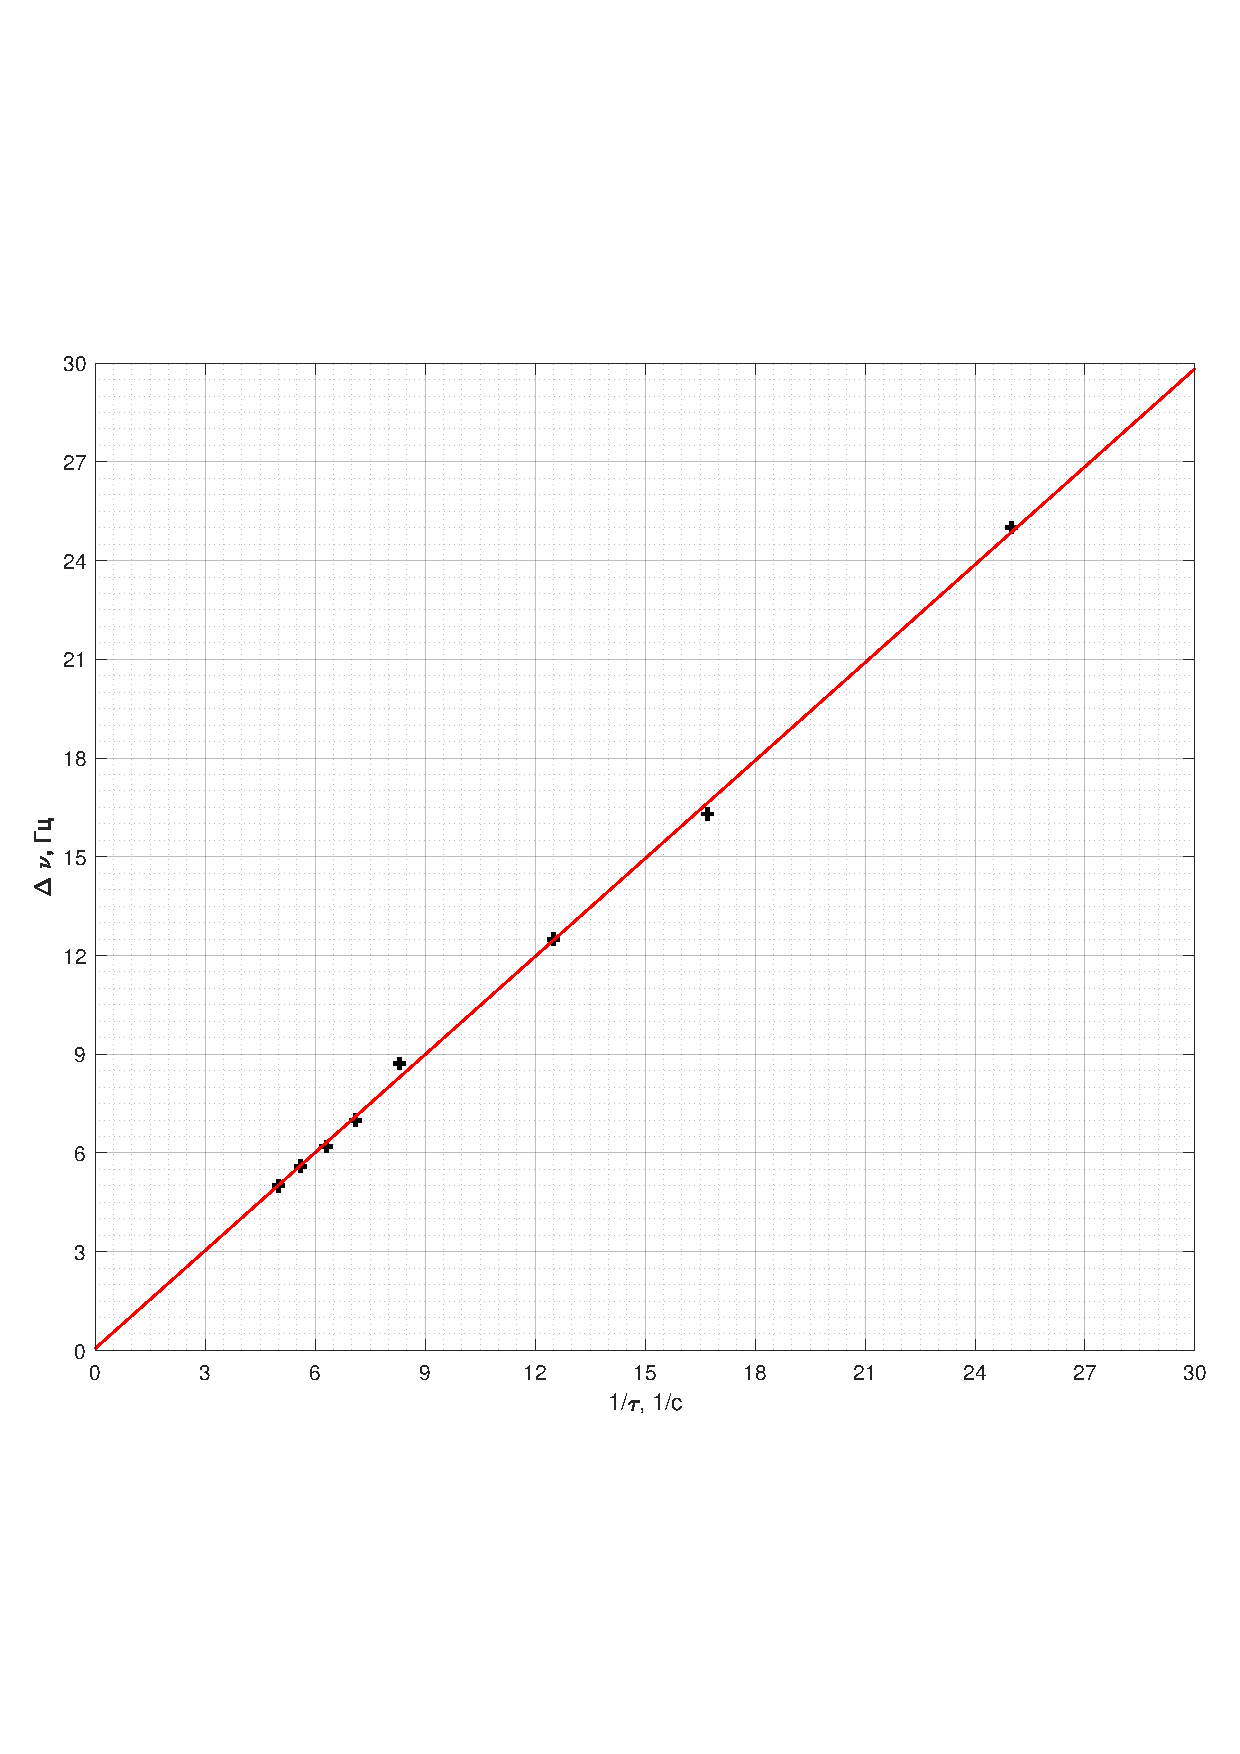
\includegraphics[width=\linewidth]{gr1.pdf}
	\caption{график зависимости $B(I)$}
\end{figure}
\end{center}

Проведем измерения по методу Гюи сначала для образца из алюминия, а потом из меди. В таблицу 2 занесём данные для меди, в таблицу 3 -- для алюминия. $\Delta m = 2$ мг - указана на весах $\Ra \Delta (\Delta P) = \Delta m \cdot 9.8 \dfrac{\text{м}}{c^2} = 19.6$ мкН $\approx 20$ мкН. $B^2$ берём из градуировки, $\Delta(B^2) = \sqrt{2}\Delta B \approx 0.02$ Тл

\begin{center}
	\begin{tabular}{|c|c|c|c|c|c|c|c|c|c|}
		\hline
		$I$, A & 1.40 & 1.60 & 1.80 & 2.00 & 2.20 & 2.40 & 2.60 & 2.80 & 3.05 \\
		\hline
		$\Delta I$, А & 0.03 & 0.03 & 0.03 & 0.03 & 0.03 & 0.03 & 0.03 & 0.03 & 0.04 \\
		\hline
		$B^2$, Тл & 0.20 & 0.26 & 0.33 & 0.40 & 0.48 & 0.57 & 0.67 & 0.77 & 0.91 \\
		\hline
		$m$, мг & 2 & 4 & 5 & 7 & 10 & 12 & 14 & 15 & 18 \\
		\hline
		$\Delta P$, мкН & 20 & 39 & 49 & 69 & 98 & 118 & 137 & 147 & 176 \\
		\hline
	\end{tabular}
	\captionof{table}{результаты измерений для меди}
\end{center}

\begin{center}
	\begin{tabular}{|c|c|c|c|c|c|c|c|c|c|c|c|c|c|}
		\hline
		$I$, A & 0.40 & 0.60 & 0.80 & 1.00  & 1.20 & 1.40 & 1.60 & 1.80 & 2.00 & 2.20 & 2.40 & 2.60 & 2.80 \\
		\hline
		$\Delta I$, А & 0.02 & 0.02 & 0.02 & 0.03 & 0.03 & 0.03 & 0.03 & 0.03 & 0.03 & 0.03 & 0.03 & 0.03 & 0.03 \\
		\hline
		$B^2$, Тл & 0.02 & 0.04 & 0.07 & 0.11 & 0.15 & 0.20 & 0.26 & 0.33 & 0.40 & 0.48 & 0.57 & 0.67 & 0.77 \\
		\hline
		$m$, мг & 1 & 2 & 3 & 7 & 9 & 13 & 16 & 21 & 25 & 30 & 35 & 39 & 43\\
		\hline
		$\Delta P$, мкН & 10 & 20 & 29 & 69 & 88 & 127 & 157 & 206 & 245 & 294 & 343 & 382 & 421 \\
		\hline
	\end{tabular}
	\captionof{table}{результаты измерений для алюминия}
\end{center}

Построим графики $|\Delta P(B^2)|$, см. \ref{gra2}

\begin{center}
	\begin{figure}[bhtp]
		\centering
		\includegraphics[width=1.05\linewidth]{gr2.pdf}
		\caption{графики зависимости $|\Delta P(B^2)|$ для алюминия и меди}\label{gra2}
	\end{figure}
\end{center}

По МНК находим, что: \[k_1 = (223 \pm 44)\dfrac{\text{мкН}}{\text{Тл}^2}, \ \ k_2 = (575 \pm 130)\dfrac{\text{мкН}}{\text{Тл}^2}\]


По формуле (4) рассчитаем магнитную восприимчивость меди и алюминия, погрешностью измерения площади образца $s$ пренебрегаем, поэтому $\sigma_\chi \approx \sigma_k$:

\[\chi_{\text{м}} = (-7.1 \pm 1.4) \cdot 10^{-6}, \ \  \chi_{\text{а}} = (18.4 \pm 4.2) \cdot 10^{-6}\]


(табличные значения для этих материалов: $\chi_{\text{м}} = -10.3 \cdot 10^{-6}, \ \  \chi_{\text{а}} = 23 \cdot 10^{-6}$)

\section*{Выводы}
\begin{enumerate}
	\item В ходе выполнения работы были расчитаны значения магнитной восприимчивости меди и алюминия: $\chi_{\text{м}} = (-7.1 \pm 1.4) \cdot 10^{-6}, \  \chi_{\text{а}} = (18.4 \pm 4.2) \cdot 10^{-6}$, которые получились немного меньше, нежели их табличные значения
	\item Большая погрешность (20\% для меди и 23\% для алюминия) получилась вследствие больших неточностей в измерениях (особенно весов).
	\item Так как $\chi_{\text{м}} < 0$, а $\chi_{\text{а}} > 0$, можно сделать вывод, что медь -- это диамагнетик, а алюминий -- это парамагнетик.
\end{enumerate}


\end{document}